\documentclass[12pt, a4paper]{article}
\usepackage[utf8]{inputenc}
\usepackage[T1]{fontenc}
\usepackage{pgfplots}
\usepackage{tikz}
\usetikzlibrary{angles}
\usetikzlibrary{quotes}
\usepackage{amssymb}
\usepackage{amsmath}
\usepackage{array}
\usepackage{amsfonts}
\usepackage{graphicx}
\usepackage{microtype}
\DeclareMathOperator{\tg}{tg}
\newcommand{\tgx}{\tg x}
\DeclareMathOperator{\ctg}{ctg}
\newcommand{\ctgx}{\ctg x}
\pgfplotsset{compat=1.18, width=10cm}

\begin{document}
\tableofcontents

\newpage
\section{Wprowadzenie do Rachunku Różniczkowego}
\subsection{Algebra}


\subsubsection{Wartość Bezwzględna}
Dla liczby x, wartość bezwzględna oznacza:
$$
|x| =
\begin{cases}
  x & \text{jeśli } x \geq 0, \\
  -x & \text{jeśli } x < 0.
\end{cases}
$$
Wartości bezwzględne posiadają również własne własności:

$$\sqrt{a^2} = \left|a\right|$$
$$\left|a\right|^2 = a^2$$
$$\left|a \cdot b\right| = \left| a \right| \cdot \left| b \right|$$
$$\left|\frac{a}{b}\right| = \frac{\left|a\right|}{\left|b\right|}$$
$$\left|a\right|=\left|b\right| \Longleftrightarrow a=b \wedge a = -b$$
Obliczanie odległości dla dwóch liczb na osi liczbowej:
$$\left|a-b\right|$$
$$\left|b-a\right|$$
Obliczanie punkty równoległego dla punktów $a$ i $b$:
$$p = \frac{a+b}{2}$$


\subsubsection*{Równania z wartością bezwzględną}
Równanie z wartością bezwględną takie jak np. $\left|x-2\right|=5$ można rozwiązać na 3 sposoby:
\begin{itemize}
  \item Sposób algebraiczny:
      $$\left|x-2\right|=5$$
      $$x-2=5 \vee x-2=-5$$
      $$x=7\vee x=-3$$
    \item Sposób geometryczny:
    \begin{center}
      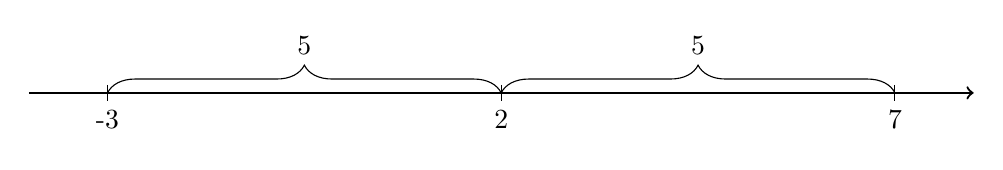
\begin{tikzpicture}
        \draw[thick, ->] (-4, 0) -- (8, 0);

        \foreach \x in {-3, 2, 7} {
          \draw (\x, 0.1) -- (\x, -0.1);
          \node[below] at (\x, -0.1) {\x};
        }
        \draw [decorate,decoration={brace,amplitude=10pt}] (-3,0) -- (2,0) node[midway,yshift=17pt] {5};
        \draw [decorate,decoration={brace,amplitude=10pt}] (2,0) -- (7,0) node[midway,yshift=17pt] {5};
        \node at (0, -0.5) {};
        \node at (0, 0.5) {};
      \end{tikzpicture}
    \end{center}
\end{itemize}
Warto pamiętać aby \textbf{nie liczyć} równań z wartością bezwzględną gdzie wynik jest ujemny, np.
$$\left|x-2\right|\neq-5$$

\subsubsection*{Równania z zagnieżdzoną wartością bezwględną}
Równanie trzeba rozbić na 2 mniejsze opuszczając przy tym wartość bezwglę\-dną, np.
$$\left|\left|x+2\right|-6\right|=1$$
\begin{align*}
\left|x+2\right|-6=1 \quad & \vee \quad \left|x+2\right|-6=-1 \\
\left|x+2\right|=7 \quad & \vee \quad \left|x+2\right|=5 \\
x+2=7 \vee x+2=-7 \hspace{1em} & \vee \hspace{1em} x+2=5 \vee x+2=-5
\end{align*}
$$x \in \left\{ -9, -7, 3, 5\right\}$$


\subsubsection*{Równania z wartością bezwględną i x}
Dla przykładowego równania $\left|x-6\right|=3x+2$ trzeba rozpatrzyć 2 przypadki:
$$x \in \left( -\infty , 6\right) \quad \cup \quad x \in \left\langle 6, +\infty \right)$$
Użyteczna jest oś liczbowa aby wyznaczyć 2 przypadki.
    \begin{center}
      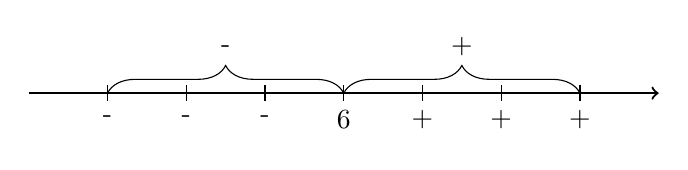
\begin{tikzpicture}
        \draw[thick, ->] (-4, 0) -- (4, 0);
        \foreach \x in {1, 2, 3} {
          \draw (\x, 0.1) -- (\x, -0.1);
          \node[below] at (\x, -0.1) {+};
        }
        \foreach \x in {-3, -2, -1} {
          \draw (\x, 0.1) -- (\x, -0.1);
          \node[below] at (\x, -0.1) {-};
        }
        \draw(0, 0.1) -- (0, -0.1);
        \node[below] at (0, -0.1) {6};
        \draw [decorate,decoration={brace,amplitude=10pt}] (-3,0) -- (0,0) node[midway,yshift=17pt] {-};
        \draw [decorate,decoration={brace,amplitude=10pt}] (0,0) -- (3,0) node[midway,yshift=17pt] {+};
        \node at (0, -0.5) {};
        \node at (0, 0.5) {};
     \end{tikzpicture}
    \end{center}
Dla przedziału liczb mniejszych wartość bezwględną mnożymy przez $-1$, a dla większych zostawiamy.
\begin{align*}
x \in \left( -\infty , 6\right) \quad & \cup \quad x \in \left\langle 6, +\infty \right) \\
-x+6=3x+2 \quad & \vee \quad x-6=3x+2 \\
-4x = -4 \quad & \vee \quad -2x = 8 \\
x = 1 \quad & \vee \quad x = -4 \notin \left\langle6, +\infty\right)
\end{align*}


\subsubsection*{Nierówności z wartością bezwzględną}
\begin{itemize}
  \item Sposób algebraiczny dla równania $\left|x + 2\right| \leq 7$. Dla znaków $<$ i $\leq$ rozdzielone równanie będzie
    koniunkcją $\wedge$ (i), natomiast dla $>$ i $\geq$ równania będą alternatywą $\vee$ (lub).
      $$\left| x+2 \right| \leq 7$$
      $$x+2 \leq 7 \wedge x+2\geq -7$$
      $$x \leq 5 \wedge x \geq -9$$
      $$x \in \langle -9,5 \rangle$$

      $$\left| x-7 \right| > 2$$
      $$x-7 > 2 \vee x-7 < -2$$
      $$x > 9 \vee x < 5$$
      $$x \in \left(-\infty, 5\right) \cup \left(9, +\infty \right)$$
  \item Sposób geometryczny dla równania $\left|x + 2\right| \leq 7$
    \begin{center}
      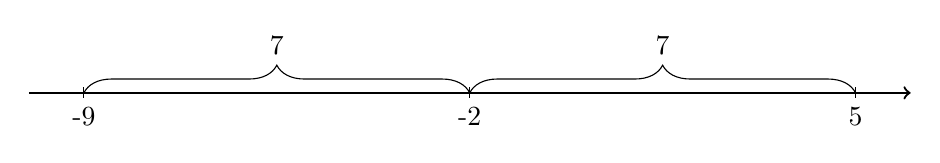
\begin{tikzpicture}[scale=0.7]
        \draw[thick, ->] (-10, 0) -- (6, 0);
        \foreach \x in {-9, -2, 5} {
          \draw (\x, 0.1) -- (\x, -0.1);
          \node[below] at (\x, -0.1) {\x};
        }
        \draw [decorate,decoration={brace,amplitude=10pt}] (-9,0) -- (-2,0) node[midway,yshift=17pt] {7};
        \draw [decorate,decoration={brace,amplitude=10pt}] (-2,0) -- (5,0) node[midway,yshift=17pt] {7};
        \node at (0, -0.5) {};
        \node at (0, 0.5) {};
     \end{tikzpicture}
    \end{center}
\end{itemize}
$$x \in \langle-9, 5\rangle$$
Przykładowe nierówności dla poszczególnych wyników:
$$\left|x\right|\geq0 \quad x \in \mathbb{R}$$
$$\left|x\right|<0 \quad x \in \varnothing$$
$$\left|x - y\right|\leq0 \quad x \in \left\{y\right\}$$


\subsubsection*{Nierówności z zagnieżdzoną wartością bezwzględną}
Nierówności z zagnieszczoną wartością bezwzględną np. $$\left|\left|x+2\right|-4\right|<10$$ działają na tej samej zasadzie co
zwykłe nierówności tylko, że rozbite na jeszcze drugą część. Dalej trzeba pamiętąc o znakach $\wedge$ i $\vee$, oraz zamiane liczby na przeciwną.

\subsubsection{Przesunięcie równoległe i symetralne funkcji wzdłuż osi OX i OY}
\subsubsection*{Przesunięcie równoległe wzdłuż osi OX i OY}
Przesunięcie wykresu funkcji najłatwiej jest zapisywać w postaci wektora przesunięcia:
$$\overrightarrow{u} = [1,5]$$
$$\overrightarrow{w} = [-2,-4]$$
Wektor $\overrightarrow{u} = [1,5]$ oznacza przesunięcie wykresu funkcji o 1 jednostke w prawą stronę
i 5 jednostki do góry, natomiast wektor $\overrightarrow{w} = [-2,-4]$
oznacza przesunięcie o jednostek 2 do lewej i 4 jednostki w dół. Na wykresie poniżej zostało przedstawione przesunięcie funkcji o
wektor $\overrightarrow{u} = [1,5]$.
\begin{center}
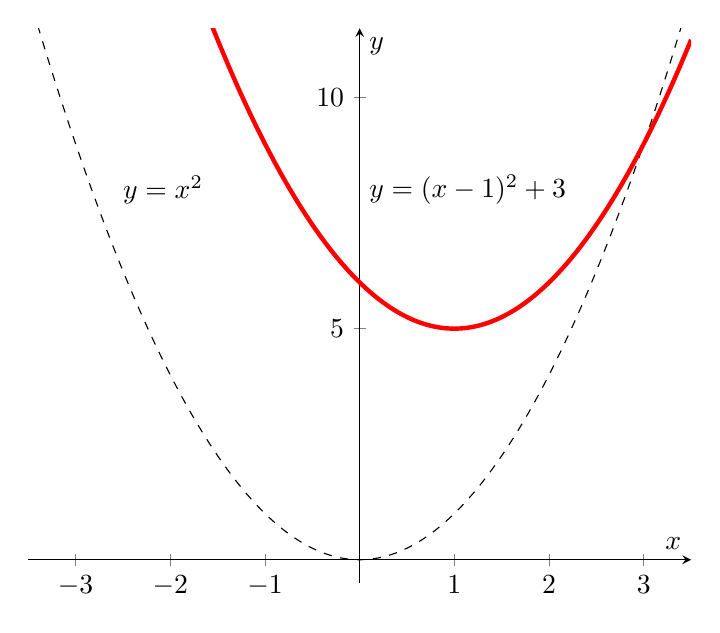
\begin{tikzpicture}
\begin{axis}[xmin=-3.5,xmax=3.5,ymin=-0.5,ymax=11.5,axis lines=middle,
            xtick={-4,-3,...,4},ytick={0,5,10}, xlabel=$x$, ylabel=$y$,
            ]
    \addplot[domain=-3.5:3.5, samples=250, dashed, black] {x^2};
    \node[anchor=west, black] at (axis cs:-2.6,8) {$y = x^2$};
    \addplot[domain=-3.5:3.5, samples=250, ultra thick, red] {(x-1)^2 + 5};
    \node[anchor=west, black] at (axis cs:0,8) {$y = (x-1)^2 + 3$};
\end{axis}
\end{tikzpicture}
\end{center}
Ogólny wzór przesunięcia funkcji o wektor $\overrightarrow{v} = [p, q]$ to:
$$g(x) = f\left(x - p\right) + q$$
\subsubsection*{przekształcenie symetralne względem osi ox i oy}
Jeżeli wykres funkcji $y=f(x)$ odbijem symetrycznie względem osi $OX$, otrzymamy wykres funkcji $$y=-f(x)$$
\begin{center}
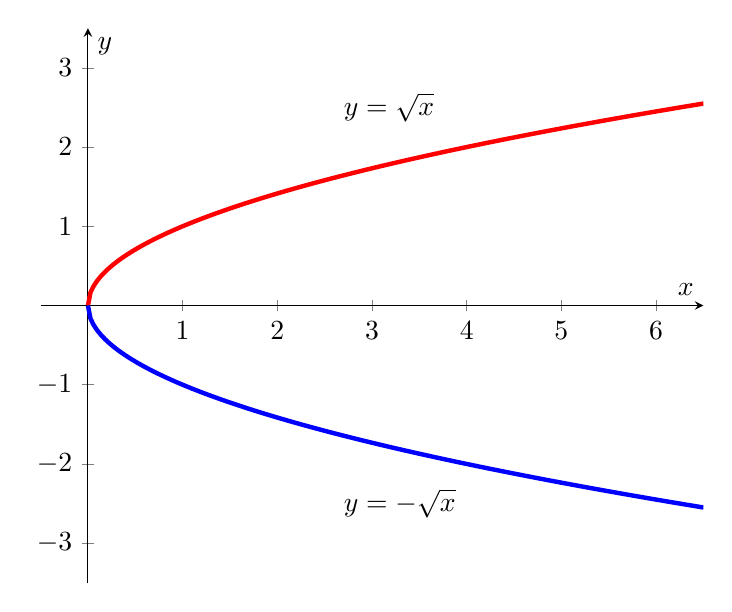
\begin{tikzpicture}
\begin{axis}[xmin=-0.5,xmax=6.5,ymin=-3.5,ymax=3.5,axis lines=middle,
            xtick={-10,...,10},ytick={-6,...,10}, xlabel=$x$, ylabel=$y$,
            ]
    \addplot[domain=0:6.5, samples=250, ultra thick, red] {sqrt(x)};
    \node[anchor=west, black] at (axis cs:2.6,2.5) {$y = \sqrt{x}$};
    \addplot[domain=0:6.5, samples=250, ultra thick, blue] {-sqrt(x)};
    \node[anchor=west, black] at (axis cs:2.6,-2.5) {$y = -\sqrt{x}$};
\end{axis}
\end{tikzpicture}
\end{center}
Jeżeli wykres funkcji $y=f(x)$ odbijem symetrycznie względem osi $OY$, otrzymamy wykres funkcji $$y=f(-x)$$
\begin{center}
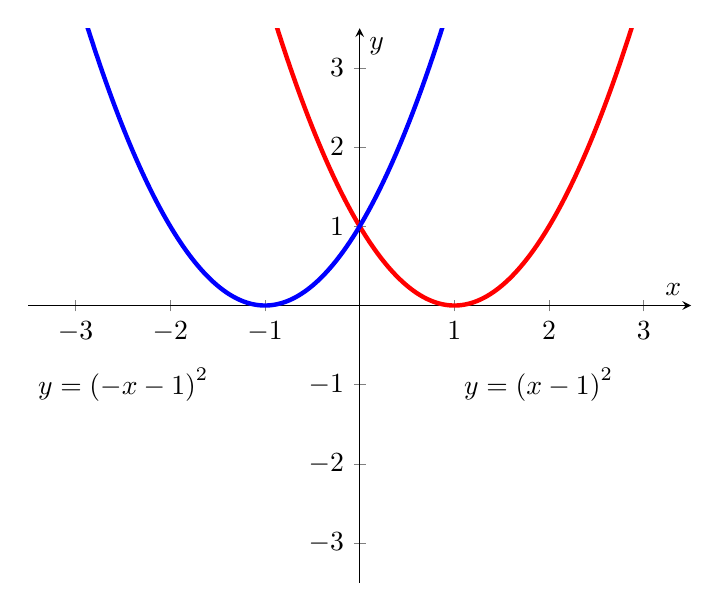
\begin{tikzpicture}
\begin{axis}[xmin=-3.5,xmax=3.5,ymin=-3.5,ymax=3.5,axis lines=middle,
            xtick={-10,...,10},ytick={-6,...,10}, xlabel=$x$, ylabel=$y$,
            ]
    \addplot[domain=-3:3, samples=250, ultra thick, red] {(x-1)^2};
    \node[anchor=west, black] at (axis cs:1,-1) {$y = \left(x-1\right)^2$};
    \addplot[domain=-3:3, samples=250, ultra thick, blue] {(-x-1)^2};
    \node[anchor=west, black] at (axis cs:-3.5,-1) {$y = \left(-x-1\right)^2$};
\end{axis}
\end{tikzpicture}
\end{center}
\subsubsection{Funkcja Kwadratowa}

\subsubsection*{Postać kanoniczna}
Funkcja kwadratowa w postaci kanonicznej to taka która ma wzór:
$$y = a(x - p)^2 + q$$
gdzie: $a \neq 0$ oraz $[p, q]$ to przesunięcie równoległe wykresu.

\subsubsection*{Postać ogólna}
Funkcja kwadratowa w postaci ogólnej to taka która ma wzór:
$$y = ax^2 + bx + c$$
gdzie: $a \neq 0$ oraz $a, b, c \in \mathbb{R}$. Przykładowa funkcja kwadratowa została przedstawiona
poniżej, wzór jej to: $y = 2x^2 + 3x + 2$
\begin{center}
\begin{tikzpicture}
\begin{axis}[xmin=-4.5,xmax=4.5,ymin=-0.5,ymax=4.5,axis lines=middle,
            xtick={-4,-3,...,4},ytick={-4,-3,...,4}, xlabel=$x$, ylabel=$y$,
            ]
  \addplot[domain=-4:4, samples=250, ultra thick,blue, ->]{2 * x^2 + 3 * x + 2};
\end{axis}
\end{tikzpicture}
\end{center}
\subsubsection*{Podstawowy opis i własności funkcji}
Wyróżnik $\Delta$ (delta) trójmianu kwadratowego: $ax^2 + bx + c$ to:
$$\Delta = b^2 - 4ac$$
Dzięki wyróznikowi $(\Delta)$ można wyznaczyć miejsca zerowe. Ilośc miejsc zerowych zależy od delty.
Jeżeli $\Delta > 0$ to funkcja posiada 2 miejsca zerowe:
$$x_0 = \frac{-b - \sqrt{\Delta}}{2a}\quad\vee\quad x_0=\frac{-b + \sqrt{\Delta}}{2a}$$
Natomiast jeżeli $\Delta = 0$ to funkcja posiada jedno miejsce zerowe:
$$x_0 = \frac{-b}{2a}$$
Dla $\Delta < 0$ funkcja nie przyjmuje miejsc zerowych (Brak rozwiązania). \\
Parabola funkcji kwadratowej posiada wierzchołek w punkcie $W=(p, q)$, gdzie:
$$p = \frac{-b}{2a}$$
$$q = \frac{-\Delta}{4a}\quad\vee\quad q = f(p)$$
Ramiona paraboli skierowane są:
$$\text{W góre dla: } a > 0$$
$$\text{W dół dla: } a < 0$$
Oś symetri paraboli to: $x = p$ \\
Punkt przecięcia z OY, posiada współrzędne $\left(0, c\right)$
\subsubsection*{Postać iloczynowa}
Funkcja kwadratowa w postaci iloczynowej istnieje jeżeli $\Delta \geq 0$ i posiada wzór:
$$y = a\left(x - x_1\right)\left(x - x_2\right)$$
gdzie: $x_1$ i $x_2$ to miejsca zerowe funkcji kwadratowej.

\subsubsection*{Równania kwadratowe}
Równania kwadratowe polegają na obliczeniu miejsc zerowych dla funkcji kwadratowej o postaci:
$$ax^2 + bx + c = 0 $$
gdzie: $a, b, c \in \mathbb{R}, a \neq 0$ \\
\vspace{0em}

\noindent Najczęstszy schemat w równaniu kwadratowym to \textbf{wzór skróconego mnożenia} i
tworzenie nowych zmiennych (np. $a = x^2, a \geq 0$) na potrzebe obliczenia równania.

\subsubsection*{Nierówności kwadratowe}
Nierówność kwadratowa to taka o postaci:
$$ax^2 + bx + c > 0$$
gdzie: $a, b, c \in \mathbb{R}, a \neq 0$ \\
Znak nierówności to $<, >, \leq, \geq$ \\
\vspace{0em}

\noindent Rozwiązując nierówność kwadratową powinno się:
\begin{itemize}
  \item Wyznaczyć miejsca zerowe dla $f(x) = ax^2 + bx + c$
  \item Naszkicować wykres funkcji $f(x)$
  \item Odczytać z wykresu funkcji rozwiązanie nierówności
\end{itemize}

\subsubsection*{Funkcje kwadratowe z wartością bezwględną}
Aby narysować wykres funkcji, należy rozważyć dwa przypadki:
$$
|x-y|=
\begin{cases}
  -(x - y) & \text{dla } x < y \\
  x - y & \text{dla } x \geq y
\end{cases}
$$
lub zapis w postaci przedziałów:
$$
x \in \left(-\infty, y\right) \vee x \in \left\langle y, +\infty \right)
$$
Wykres tej funkcji bedzię składał się z $2$ części, kończące się i rozpoczynające się w punkcie $y$.
Najłatwiej wyznaczyć wierzchołek $\left(p, q\right)$ i naszkicować funkcje.
Przykład dla funkcji $f(x) = x|x-1|$
\begin{center}
\begin{tikzpicture}
\begin{axis}[xmin=-4.5,xmax=4.5,ymin=-2.5,ymax=2.5,axis lines=middle,
            xtick={-4,-3,...,4},ytick={-4,-3,...,4}, xlabel=$x$, ylabel=$y$,
            ]
  \addplot[domain=-4:4, samples=250, ultra thick,blue, ->]{abs(x - 1) * x};

  \draw[dashed] (axis cs:1,-4) -- (axis cs:1,4);
\end{axis}
\end{tikzpicture}
\end{center}

\subsubsection*{Wzory Viete'a}
Jeżeli funkcja $f(x) = ax^2 + bx + c$ ma 2 miejsca zerowe $x_1 i x_2$ $(\Delta \geq 0)$, to zachodzą wzory Viete'a:
$$x_1 + x_2 = -\frac{b}{a}$$
$$x_1x_2 = \frac{c}{a}$$
Dzięki wzorą Viete'a można określić jakie znaki mają miejsca zerowe (Różne, dodatnie lub ujemne). Schematem najczęsciej
pojawiającym się w wzorach Viete'a to wzory skróconego mnożenia do pewnego stopnia.
\subsection{Trygonometria}
W $\triangle$ prostokątnym dany jest kąt $\theta$. Wyraża się 4 funkcje trygonometryczne:
$$\sin\theta=\frac{a}{c}$$
$$\cos\theta=\frac{b}{c}$$
$$\tg\theta=\frac{a}{b}$$
$$\ctg\theta=\frac{b}{a}$$
\begin{center}
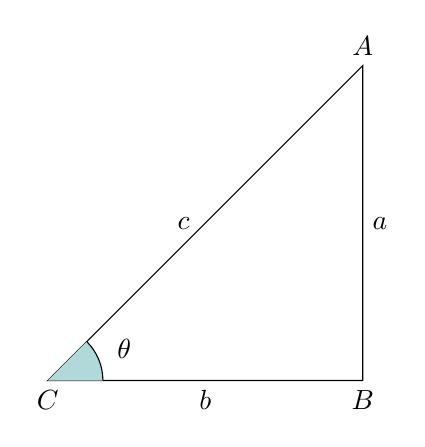
\begin{tikzpicture}
  \draw (0,0) coordinate[label=below:$C$] (c) --
        (4,0) coordinate[label=below:$B$] (b) node[midway, below] {$b$} --
        (4,4) coordinate[label=above:$A$] (a) node[midway, right] {$a$} --
        cycle node[midway, left=0.075cm] {$c$};
      \pic[draw, fill=teal!30, angle radius=7mm, "$\theta$", angle eccentricity=1.5] {angle = b--c--a};
\end{tikzpicture}
\end{center}
Funkcje trygonometryczne również posiadają tożsamości trygonometryczne takie jak np.
$$\sin^2\theta+\cos^2\theta = 1$$
$$\tg\theta=\frac{\sin\theta}{\cos\theta}$$
$$\ctg\theta=\frac{\cos\theta}{\sin\theta}$$
$$\tg\theta\cdot\ctg\theta=1$$
Funkcje trygonometryczne można konwertować na inne funkcje:
$$\sin(90^{\circ}-\theta)=\cos\theta$$
$$\cos(90^{\circ}-\theta)=\sin\theta$$
$$\tg(90^{\circ}-\theta)=\ctg\theta$$
$$\ctg(90^{\circ}-\theta)=\tg\theta$$
\section{Rachunek różniczkowo-całkowy}
\section{Algebra liniowa}
\subsection{Wektory}
Wektor to uporządkowana para liczb. Jeśli wektor ma początek to jest to, wektor
zaczepiony który jest oznaczany symbolem $\overrightarrow{AB}$. Jeżeli dane są punkty
$A = (x_1,y_1)$ oraz $B = (x_2,y_2)$,
to współrzędne wektora $\overrightarrow{AB}$ określa wzór: $$\overrightarrow{AB} = [x_2-x_1,y_2-y_1]$$
Jeśli natomiast wektor nie ma początku to jest to wektor swobodny który
jest oznaczany symbolem $\overrightarrow{v}, \overrightarrow{u}, \overrightarrow{w}$.
$$\overrightarrow{u} = \overrightarrow{w} \Longleftrightarrow u_x = w_x \wedge u_y = w_y$$
Na rysunku poniżej został przedstawiony wygląd wektora $[3,2]$ i $[-2,4]$ w układzie współrzędnych:

\begin{center}
\begin{tikzpicture}
\begin{axis}[xmin=-4.5,xmax=4.5,ymin=-2.5,ymax=4.5,axis lines=middle,
            xtick={-4,-3,...,4},ytick={-4,-3,...,4}, xlabel=$x$, ylabel=$y$,
            ]
  \addplot[domain=0:4, samples=250, ultra thick,blue, ->] coordinates {
    (0,0)
    (3,2)
  }
  node[pos=1.0, above left, blue]{$[3,2]$};
  \addplot[domain=0:4, samples=250,dashed] coordinates {
    (0,2)
    (3,2)
    (3,0)
  };

  \addplot[domain=0:4, samples=250, ultra thick,red, ->] coordinates {
    (0,0)
    (-2,4)
  }
  node[pos=1.0, below left, red]{$[-2,4]$};
  \addplot[domain=0:4, samples=250,dashed] coordinates {
    (0,4)
    (-2,4)
    (-2,0)
  };

\end{axis}
\end{tikzpicture}
\end{center}
Długość wektora $\overrightarrow{w}$ oraz $\overrightarrow{AB}$ można zapisać następująco:
$$|\overrightarrow{w}| = \sqrt{w^2_x + w^2_y}$$
$$|\overrightarrow{AB}| = \sqrt{\left(x_2 - x_1\right)^2 \left(y_2 - y_1\right)^2}$$
gdzie:
\begin{itemize}
  \item $A(x_1,y_1)$ i $B(x_2,y_2)$ to długości wektora $\overrightarrow{AB}$
\end{itemize}
\vspace{1em}
Sumą, różnicą, iloczynem $\overrightarrow{u} = [u_x,u_y]$ i $\overrightarrow{w} = [w_x,w_y]$, wyraża się wzorem:
$$\overrightarrow{u} + \overrightarrow{w} = [u_x + w_x, u_y + w_y]$$
\begin{center}
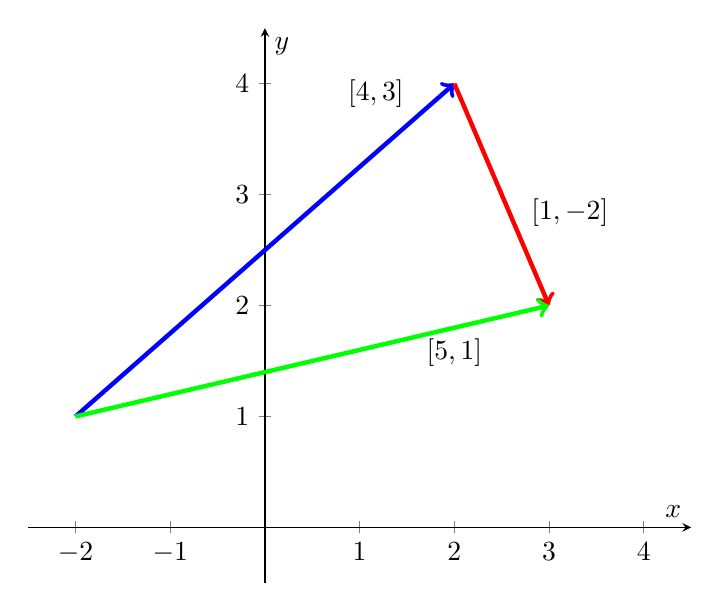
\begin{tikzpicture}
\begin{axis}[xmin=-2.5,xmax=4.5,ymin=-0.5,ymax=4.5,axis lines=middle,
            xtick={-4,-3,...,4},ytick={-4,-3,...,4}, xlabel=$x$, ylabel=$y$,
            ]
  \addplot[domain=0:4, samples=250, ultra thick,blue, ->] coordinates {
    (-2,1)
    (2,4)
  }
  node[pos=1.0, above = -0.125cm, left = 0.50cm, black]{$[4,3]$};
  \addplot[domain=0:4, samples=250, ultra thick,red, ->] coordinates {
    (2,4)
    (3,2)
  }
  node[pos=0.9, above = 0.9cm, right = -0.25cm, black]{$[1,-2]$};
  \addplot[domain=0:4, samples=250, ultra thick,green, ->] coordinates {
    (-2,1)
    (3,2)
  }
  node[pos=0.8, below, black]{$[5,1]$};
\end{axis}
\end{tikzpicture}
\end{center}
$$\overrightarrow{u} - \overrightarrow{w} = [u_x - w_x, u_y - w_y]$$

\begin{center}
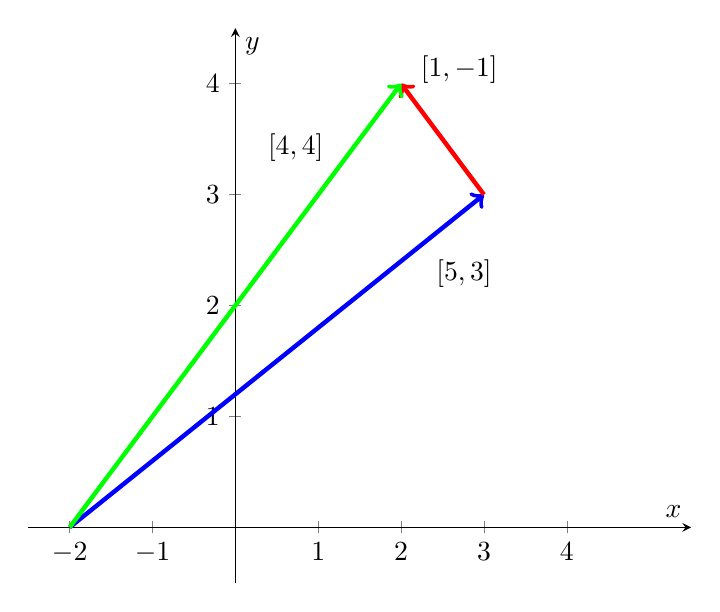
\begin{tikzpicture}
\begin{axis}[xmin=-2.5,xmax=5.5,ymin=-0.5,ymax=4.5,axis lines=middle,
            xtick={-4,-3,...,4},ytick={-4,-3,...,4}, xlabel=$x$, ylabel=$y$,
            ]
  \addplot[domain=0:4, samples=250, ultra thick,blue, ->] coordinates {
    (-2,0)
    (3,3)
  }
  node[pos=1.0, below = 1cm, right = -0.75cm, black]{$[5,3]$};

  \addplot[domain=0:4, samples=250, ultra thick,red, ->] coordinates {
    (3,3)
    (2,4)
  }
  node[pos=0.9, above right, black]{$[1,-1]$};

  \addplot[domain=0:4, samples=250, ultra thick,green, ->] coordinates {
    (-2,0)
    (2,4)
  }
  node[pos=0.8, above left, black]{$[4,4]$};
\end{axis}
\end{tikzpicture}
\end{center}
$$ a \cdot \overrightarrow{w} = [a \cdot w_x, a \cdot w_y], \quad \text{gdzie } a \in \mathbb{R}$$
\begin{center}
\begin{tikzpicture}
\begin{axis}[xmin=-3.5,xmax=2.5,ymin=-3.5,ymax=2.5,axis lines=middle,
            xtick={-4,-3,...,4},ytick={-4,-3,...,4}, xlabel=$x$, ylabel=$y$,
            ]
  \addplot[domain=0:4, samples=250, ultra thick,blue, ->] coordinates {
    (0,0)
    (1,1)
  }
  node[pos=1.0, above right, black]{$[5,3]$};

  \addplot[domain=0:4, samples=250, ultra thick,red, ->] coordinates {
    (0,0)
    (-2,-2)
  }
  node[pos=0.9, below left = 0.25cm, black]{$[-2,-1]$};
\end{axis}
\end{tikzpicture}
\end{center}
Wektory $\overrightarrow{u} = [u_x, u_y]$ i $\overrightarrow{w} = [w_x, w_y]$, są przeciwne wtedy,
gdy suma wektorów $\overrightarrow{u}$ i $\overrightarrow{w}$ jest wektorem zerowym, czyli:
$$\overrightarrow{u} = -\overrightarrow{w} \Longleftrightarrow u_x + w_x = 0 \wedge u_y + w_y = 0$$
Iloczyn skalarny wektorów $\overrightarrow{u} = [u_1,u_2]$ i $\overrightarrow{w} = [w_1,w_2]$ to liczba, którą można uzyskać
dodając iloczyny odpowiednich współrzędnych:
$$\overrightarrow{u} \cdot \overrightarrow{w} = u_1 \cdot w_1 + u_2 \cdot w_2$$
Iloczyn skalarny wektorów można również wyliczyć znając długości wektorów $|\overrightarrow{u}|$ i $|\overrightarrow{w}|$
oraz kąt $\theta$ między nimi:
$$\overrightarrow{u} \cdot \overrightarrow{w} = |\overrightarrow{u}| \cdot |\overrightarrow{w}| \cdot \cos \theta$$
\begin{center}
\begin{tikzpicture}
\begin{axis}[xmin=-3.5,xmax=3.5,ymin=-0.5,ymax=3.5,axis lines=middle,
            xtick={-4,-3,...,4},ytick={-4,-3,...,4}, xlabel=$x$, ylabel=$y$,
            ]
  \addplot[domain=0:4, samples=250, ultra thick,blue, ->] coordinates {
    (-2,1)
    (1,3)
  }
  node[pos=1.0, below right, black]{$[3,2]$};

  \addplot[domain=0:4, samples=250, ultra thick,red, ->] coordinates {
    (-2,1)
    (3,1)
  }
  node[pos=0.9, above left, black]{$[5,0]$};
\end{axis}
\end{tikzpicture}
\end{center}

\section{Logika i Dowody matematyczne}
\subsubsection*{Symbole i ich znaczenie}
W logice matematycznej występuje duża ilość symboli matematycznych, a to one i ich znaczenie:
$$
\begin{array}{l@{\quad}l}
  \textbf{Symbol} & \textbf{Znaczenie} \\
  \hline
  \neg p, \sim p & \text{negacja p} \\
  p \wedge q & \text{p i q} \\
  p \vee q & \text{p lub q} \\
  p \Rightarrow q & \text{jeżeli p to q} \\
  p \Leftrightarrow q & \text{p tylko wtedy i tylko wtedy, gdy} \\
  \therefore & \text{zatem} \\
  \forall & \text{dla każdego} \\
  \exists & \text{istnieje takie} \\
\end{array}
$$
Negacja to zaprzeczenie wyrażania o formie: \textbf{negacja z} $P$
\begin{center}
\begin{tabular}{c@{\quad}c}
\textbf{P} & $\neg$ \textbf{P} \\ \hline
F & T \\
T & F \\
\end{tabular}
\end{center}
Alternatywa (lub) to wyrażenie o formie: $P$ \textbf{lub} $Q$.\begin{center}
\begin{tabular}{c@{\quad}c@{\quad}c}
\textbf{P} & \textbf{Q} & \textbf{P} $\vee$ \textbf{Q} \\ \hline
F & F & F \\
T & F & T \\
F & T & T \\
T & T & T \\
\end{tabular}
\end{center}
Koniunkcja (i) to wyrażenie o formie: $P$ \textbf{i} $Q$.
\begin{center}
\begin{tabular}{c@{\quad}c@{\quad}c}
\textbf{P} & \textbf{Q} & \textbf{P} $\wedge$ \textbf{Q} \\ \hline
F & F & F \\
F & T & F \\
T & F & F \\
T & T & T \\
\end{tabular}
\end{center}
Implikacja to wyrażenia o formie: \textbf{Jeżeli} $P$ \textbf{to} $Q$.
\begin{center}
\begin{tabular}{c@{\quad}c@{\quad}c}
\textbf{P} & \textbf{Q} & \textbf{P} $\Rightarrow$ \textbf{Q} \\ \hline
F & F & T \\
F & T & T \\
T & F & F \\
T & T & T \\
\end{tabular}
\end{center}
Równoważność to wyrażenia o formie: $P$ \textbf{wtedy i tylko wtedy, gdy} $Q$.
\begin{center}
\begin{tabular}{c@{\quad}c@{\quad}c}
\textbf{P} & \textbf{Q} & \textbf{P} $\Leftrightarrow$ \textbf{Q} \\ \hline
F & F & T \\
F & T & F \\
T & F & F \\
T & T & T \\
\end{tabular}
\end{center}
\subsubsection*{Prawa rachunku - wzory i definicja}
\textbf{Prawa De Morgana}
$$\neg\left(P \wedge Q\right) \Leftrightarrow \neg P \vee \neg Q$$
$$\neg\left(P \vee Q\right) \Leftrightarrow \neg P \wedge \neg Q$$
\textbf{Prawo asocjacyjne}
$$P \wedge \left(Q \wedge R\right) \Leftrightarrow \left(P \wedge Q\right) \wedge R \Leftrightarrow P \wedge Q \wedge R$$
$$P \vee \left(Q \vee R\right) \Leftrightarrow \left(P \vee Q\right) \vee R \Leftrightarrow P \vee Q \vee R$$
\textbf{Prawo idempotentności}
$$P \wedge P \Leftrightarrow P$$
$$P \vee P \Leftrightarrow P$$
\textbf{Prawo rozdzielności}
$$P \wedge \left(Q \vee R\right) \Leftrightarrow \left(P \wedge Q\right) \vee \left(P \wedge R\right)$$
$$P \vee \left(Q \wedge R\right) \Leftrightarrow \left(P \vee Q\right) \wedge \left(P \vee R\right)$$
\textbf{Prawa absorpcji}
$$P \vee \left(P \wedge Q\right) \Leftrightarrow P$$
$$P \wedge \left(P \vee Q\right) \Leftrightarrow P$$
\textbf{Prawo podwójnej negacji}
$$\neg\neg P \Leftrightarrow P$$
\subsection*{Dowody Matematyczne}

\textbf{Przypuszczenie 1.} Załóżmy, że $n \in \mathbb{Z}$, $n > 1$ i do tego nie jest liczbą pierwszą.
Wtedy $2^n - 1$ nie jest liczbą pierwszą.
\vspace{1em}

\noindent \textbf{Udowodnienie przypuszczenia 1.} Ponieważ $n$ nie jest liczbą pierwszą, istnieją liczby całkowite
dodatnie $a$ i $b$ takie, że $a < n, b < n$ i $n = ab$. Niech $x = 2^b - 1$ i $y = 1 + 2^b + 2^{2b} + \dots + 2^{\left(a-1\right)b}$.
Więc
\begin{align*}
  xy &= \left(2^b -1\right) \cdot \left(1 + 2^b + 2^{2b} + \dots + 2^{\left(a - 1\right)b}\right) \\
     &= 2^b \cdot \left(1 + 2^b + 2^{2b} + \dots + 2^{\left(a-1\right)b}\right) - \left(1 + 2^b + 2^{2b} + \dots + 2^{\left(a-1\right)b}\right) \\
     &= \left(2^b + 2^{2b} + 2^{3b} + \dots + 2^{ab}\right) - \left(1 + 2^b + 2^{2b} + \dots + 2^{\left(a - 1\right)b}\right) \\
     &= 2^{ab} - 1 \\
     &= 2^n - 1.
\end{align*}
Ponieważ $b < n$, możemy stwierdzić, że $x = 2^b - 1 < 2^n - 1$. Dodatkowo, ponieważ $ab = n > a$, wynik stąd, że $b > 1$.
Zatem, $x = 2^b - 1 > 2^1 -1 = 1$, czyli $y < xy = 2^n - 1$. Zatem, udowodniliśmy, że $2^n - 1$ można zapisać jako iloczyn
dwóch liczb dodatnich całkowitych $x$ i $y$, obie liczby są mniejsze niż $2^n - 1$, czyli $2^n - 1$ nie jest liczbą pierwszą. \hfill $\square$
\end{document}
